\chapter{Exam II (Practice)}
\label{ch:examii-practice}

\begin{cluster}
\label{grp:prmbl:examii-practice::minutes}

\begin{preamble}
\label{prmbl:examii-practice::minutes}
\begin{itemize}
\item You have 80 minutes to complete this examination.
\item Please answer all questions in the space provided with the
  question.  Clearly indicate your answers.
\item You may refer to your one double-sided $8\frac{1}{2} \times 11$in
  sheet of paper with notes, but to no other person or source, during the
  examination.

\item Your answers for this exam must be written in blue or black ink.

\end{itemize}

\end{preamble}
\end{cluster}


\section{Problem 1: True or False}
\label{sec:examii-practice::problem-1-true-or-false}


\section{Problem 2: Short Answers}
\label{sec:examii-practice::problem-2-short-answers}

\begin{cluster}
\label{grp:prb:examii-practice::classes}

\begin{problem}[4][Classes]
\label{prb:examii-practice::classes}
\used{Fall 14, Final}

Lets say you are given a table that maps every student to the set of
classes they take.  

\ask \label{prt-ask:examii-practice::fill}

Fill in the algorithm below that returns all classes,
assuming there is at least one student in each class.  Your algorithm
must run in $O(m \log n)$ work and $O((\log m)(\log n))$ span, where
$n$ is the number of students and $m$ is the sum of the number of
classes taken across all students.    Note, our solution is one line.

\begin{lstlisting}[numbers=none]
fun allClasses($T$ : classSet studentTable) : classSet = 
@\vspace{.5in}@
\end{lstlisting}


\sol \label{cki-sol:examii-practice::numbers}

\begin{lstlisting}[numbers=none]
fun allClasses($T$) = Table.reduce Set.union $\emptyset$ $T$
\end{lstlisting}

\end{problem}
\end{cluster}

\begin{cluster}
\label{grp:prb:examii-practice::shortest-weighted}

\begin{problem}[5][Shortest Weighted]
\label{prb:examii-practice::shortest-weighted}
\used{Fall 14, Practice Exam II}

Given a graph with integer edge weights between $1$ and $5$
(inclusive), you want to find the shortest \emph{weighted} path
between a pair of vertices. 

\ask \label{prt-ask:examii-practice::would}

How would you reduce this problem to the
shortest \emph{unweighted} path problem, which can be solved using
BFS?


\sol \label{cki-sol:examii-practice::replace}

Replace each edge with weight $i$ with a simple path of $i$ edges
each with weight $1$. Then solve with BFS.

\end{problem}
\end{cluster}

\begin{cluster}
\label{grp:prb:examii-practice::enter-and-exit}

\begin{problem}[5][Enter and Exit]
\label{prb:examii-practice::enter-and-exit}
 \used{Fall 14, Practice Exam II}

Recall the implementation of DFS shown in class using the \sml{enter}
and \sml{exit} functions. Circle the correct answer for each of the
following statements, assuming DFS starts at $A$:

\begin{center}
  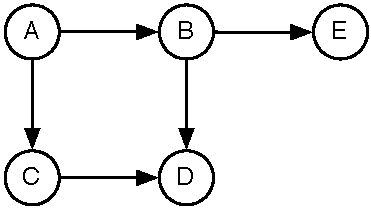
\includegraphics[scale=.7]{dfs/dfs-graph1.pdf}
\end{center}

\bigskip
  \begin{tabular}{lp{1.3in}cc}
    \texttt{enter D} could be called before \texttt{enter E}:& &
    \textsf{True} & \textsf{False}\\[1.5 ex]
    \texttt{enter E} could be called before \texttt{enter D}:& & \textsf{True} & \textsf{False}\\[1.5 ex]
    \texttt{enter D} could be called before \texttt{enter C}:& & \textsf{True} & \textsf{False}\\[1.5 ex]
    \texttt{exit A} could be called before \texttt{exit B}: & & \textsf{True} & \textsf{False}\\[1.5 ex]
    \texttt{exit D} could be called before \texttt{enter B}:&  & \textsf{True} & \textsf{False}
  \end{tabular}

\sol
    True, True, True, False, True

\end{problem}
\end{cluster}

\begin{cluster}
\label{grp:prb:examii-practice::fall}

\begin{problem}[5]
\label{prb:examii-practice::fall}
\used{Fall 14, Practice Exam II}

A new startup \emph{FastRoute} wants to route information along a path
in a communication network, represented as a graph. Each vertex
represents a router and each edge a wire between routers. The wires
are weighted by the maximum bandwidth they can
support. \emph{FastRoute} comes to you and asks you to develop an
algorithm to find the path with maximum bandwidth from any source $s$
to any destination $t$. As you would expect, the \emph{bandwidth} of a
path is the minimum of the bandwidths of the edges on that path; the
minimum edge is the \emph{bottleneck}.

\ask \label{prt-ask:examii-practice::explain}

Explain how to modify Dijkstra's algorithm to do this. In particular, how would
you change the priority queue and the following relax step?

\begin{quote}
\sml{fun relax (Q, (u,v,w)) = PQ.insert (d(u) + w, v) Q}
\end{quote}

Justify your answer.


\sol \label{cki-sol:examii-practice::priority}

  We'll use a max priority queue instead of a min priority queue used
  in Dijkstra's. We will also modify the relax step to insert into the
  priority queue $\min(d(u), w)$ because the quality of a path is the
  minimum of the edge weights. These changes don't affect the
  correctness of Dijkstra's, so we could explore the vertices like in
  Dijkstra's.

\end{problem}
\end{cluster}

\begin{cluster}
\label{grp:prb:examii-practice::parallel-cycle-detection}

\begin{problem}[4][Parallel Cycle Detection]
\label{prb:examii-practice::parallel-cycle-detection}


\ask \label{prt-ask:examii-practice::describe}

Describe in words how you would as part of star contraction 
efficiently detect that an undirected graph has a cycle.  \textbf{No more than two sentences.}


\sol \label{cki-sol:examii-practice::star}

If during star contraction we find any self edges not involved in
contraction itself then there is a cycle.   However,
we need to be careful not to remove duplicate edges, and only to
contract along a single duplicate edge.

-4 if claim detecting duplicate edges is sufficient.  It is not sufficient because you can contract duplicate edges at the same time\\
-2 if say detect self edge, but do not point out issue with duplicates.\\
0 for DFS, BFS, etc.

\end{problem}
\end{cluster}

\begin{cluster}
\label{grp:prb:examii-practice::star-contraction}

\begin{problem}[6][Star Contraction]
\label{prb:examii-practice::star-contraction}


\ask \label{prt-ask:examii-practice::circle}

Circle \textbf{every} type of graph listed below for which star
contraction will reduce the number of \textbf{edges} by a constant
factor in expectation in every round until fully reduced (and hence
imply $O(|E|)$ total work).  You can assume redundant edges between
vertices are removed.\\

(a) a graph in which all vertices have degree at most 2\\
(b) a graph in which all vertices have degree at most 3\\
(c) a graph in which all vertices have degree $\sqrt{|V|}$\\
(d) a graph containing a single cycle (i.e. a forest with one additional edge)\\
(e) the complete graph (i.e. an edge between every pair of vertices)\\
(f) any graph (still circle others if relevant)\\


\sol \label{cki-sol:examii-practice::_1_}

a, d, e

\end{problem}
\end{cluster}

\begin{cluster}
\label{grp:prb:examii-practice::dfs-edges}

\begin{problem}[DFS Edges]
\label{prb:examii-practice::dfs-edges}
The following questions have to do with the four types of edges in
a depth first search (DFS): \textbf{tree edges}, \textbf{back edges},
\textbf{forward edges} and \textbf{cross edges}.  For each one list
\textbf{all} types of edges that apply.

\ask \label{prt-ask:examii-practice::3pts}
[3pts]
What kind of edges can a \textbf{bridge}, as defined in AbridgedLab, be

\sol \label{cki-sol:examii-practice::tree}

tree edge

\ask[3pts]
Assume we enter $u$ before entering $v$ during the DFS, what kind of
edge can the edge $(u,v)$ (directed from $u$ to $v$) be?

\sol \label{cki-sol:examii-practice::forward}

forward edge, tree edge


\ask[3pts]
What kind of edges can appear in DFS for a directed graph in which
every edge appears in both directions (i.e. if $(u,v) \in E$ then $(v,u)
\in E$).

\sol \label{cki-sol:examii-practice::edges}

tree edges, forward edges, backward edges


\ask[3pts] Lets say that in a directed graph $u$ and $v$ are in two
different strongly connected components (in a strongly connected
component all vertices can reach all others).  What kind of edges can
be between $u$ and $v$.

\sol \label{cki-sol:examii-practice::cross}

tree edges, forward edges, cross edges

\ask[3pts]
In the topological sorting algorithm for directed acyclic graph we
described in class and the notes, lets say a vertex $u$ appears
after a vertex $v$.  What kind of edges can be in a path
from $v$ to $u$.

\sol \label{cki-sol:examii-practice::_2_}

tree edges, forward edges, cross edges


\end{problem}
\end{cluster}


\section{Problem 3: Sets and Tables}
\label{sec:examii-practice::problem-3-sets-and-tables}


\section{(Shortest Paths) Dijkstra and A*}
\label{sec:examii-practice::shortest-paths-dijkstra-and-a}

\begin{cluster}
\label{grp:grm:examii-practice::fall}

\begin{gram}
\label{grm:examii-practice::fall}
\used{Fall 14, Practice Exam II}

\end{gram}
\end{cluster}

\begin{cluster}
\label{grp:prb:examii-practice::consider}

\begin{problem}[6]
\label{prb:examii-practice::consider}
Consider the graph shown below, where the edge weights appear next to
the edges and the heuristic distances to vertex $G$ are in parenthesis
next to the vertices.
\begin{center}
  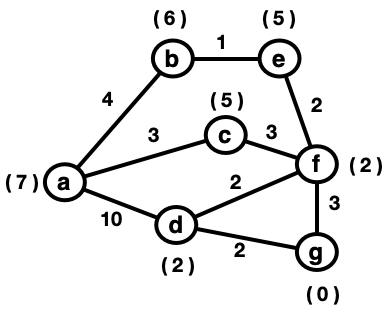
\includegraphics[scale=.75]{shortest-paths/graph}
\end{center}

\ask \label{prt-ask:examii-practice::show}

Show the order in which vertices are visited by Dijkstra when the source
vertex is $A$.

\sol \label{cki-sol:examii-practice::show}

A C B E F D G


\ask Show an order in which vertices are visited by $A^*$ when
the source vertex is $A$ and the destination vertex is $G$.


\sol \label{cki-sol:examii-practice::_3_}

A C F G 


\end{problem}
\end{cluster}

\begin{cluster}
\label{grp:prb:examii-practice::reason}

\begin{problem}[4]
\label{prb:examii-practice::reason}


\ask \label{prt-ask:examii-practice::reason}

What is the key reason you would choose to use $A^*$ instead of
Dijkstra's algorithm?


\sol \label{cki-sol:examii-practice::want}

You can use $A^*$ if you want the shortest path to only a single goal vertex,
and not all shortest paths. $A^*$ can be much more efficient, as it tries to
move toward the goal more directly, skipping many more vertices.

\end{problem}
\end{cluster}

\begin{cluster}
\label{grp:prb:examii-practice::show}

\begin{problem}[5]
\label{prb:examii-practice::show}
Show a $3$-vertex example of a graph on which Dijkstra's algorithm always
fails. Please clearly identify which vertex is the source.

\sol
\begin{verbatim}
         A 
        / \
   x=4 /   \ y=-2   x+y < z < x guarantees failure
      /     \       x+y < z <= x may fail depending on the input order
    S ------- B
        z=3
\end{verbatim}

\end{problem}
\end{cluster}

